%
% problemstellung.tex -- Problemstellung Kalman-Filter
%
% (c) 2006-2015 Prof. Dr. Andreas Mueller, Hochschule Rapperswil
%

\section{Problemstellung}
Im Einführungsbeispiel wurde ein eindimensionales System betrachtet,
welches sich nicht verändert.
Im Allgemeinen wird ein System durch
mehrere Variablen beschrieben, die sich in der Zeit verändern.
in diesem Abschnitt wollen wir die Problemstellung des eindimensionalen
Problems auf mehrdimensionale Systeme verallgemeinern.

\subsection{System und Beobachtung}
Zwei Positionsmessung im zeitlichen Abstand $\Delta t$
bei einem Fahrzeug, welches selbständig
in seiner Fahrbahn bleiben soll, können sich bis auf Messfehler um höchstens
$v\Delta t$ unterscheiden, wenn sich das Fahrzeug mit Geschwindigkeit $V(t)$
quer zur Fahrtrichtung bewegt.
Insbesondere würden wir für die zweite
Messung ungefähr den Wert $E(X(t+\Delta t)) = X(t) + V(t)\Delta t$
erwarten.
Hier haben wir unser Wissen über das System einfliessen lassen.

Offensichtlich ist es also möglich, eine gute Voraussage über den
zukünftigen Zustand $X(t+\Delta t)$ zu machen, wenn $X(t)$ und $V(t)$
bekannt sind.
Natürlich wird diese Voraussage nicht mit der tatsächlichen
Messung zur Zeit $t+\Delta t$ übereinstimmen.
Zum einen werden unweigerlich
neue Messfehler auftreten, zum anderen basiert die Voraussage ja bereits
auf Daten, die mit einem Messfehler behaftet sind.
Die Voraussage ist also
ebenfalls eine Zufallsvariable, die jedoch auf der Kenntnis eines früheren
Zustands des Systems basiert.

Wir modellieren dieses Problem jetzt für den Fall konstanter Zeitschritte.
Den Zustand des Systems betrachten wir als Vektor $x_k\in\mathbb{R}^n$,
wobei $k\in\mathbb{N}$.
Diese Vektoren sind nicht vollständig beobachtbar,
nur ein Abbild davon ist messbar.
Grundsätzlich müssten wir also eine
bestimmte Funktion auf $x_k$ anwenden, um die Messgrössen zu finden,
für die meisten praktischen Anwendungen genügt es, eine lineare Abbildung
zu verwenden.
Es gibt also eine Matrix $H_k$, welche die beobachteten
Grössen $z_k=H_kx_k$ bestimmt.

Die Zeitentwicklung des Systems muss aus einem Zustand $x_k$ den nächsten
Zustand $x_{k+1}$ berechnen.
Bei einem
einfachen System mit der Bewegungsgleichung
\[
\frac{dx(t)}{dt}=ax(t)
\]
gilt zum Beispiel $x(t_2)=e^{a(t_2-t_1)}x(t_1)$, d.~h.~der Zeitschritt
kann durch Multiplikation mit einer Zahl $e^{a\Delta t}$ berechnet werden.
ersetzt man $x$ durch einen Vektor $\vec x$ und $a$ durch eine Matrix
$A$, wird die Lösung zu $\vec x(t_2)=e^{A(t_2-t_1)}\vec x(t_1)$,
insbesondere gibt es also eine Matrix $\varphi=e^{A\Delta t}$, mit
der der aktuelle Zustand multipliziert werden muss, um den zukünftigen
Zustand zu ermitteln.
Bei genügend kleinem Zeitschritt kann man jedes
System soweit linearisieren, dass diese Annahme zutrifft, die Matrix
wird aber im Allgemeinen zeitabhängig sein.
Die Bewegungsgleichung
wird damit in linearisierter Form
\[
x_{k+1}=\varphi_kx_k.
\]

\subsection{Messfehler und Systemfehler}
\begin{figure}
\centering
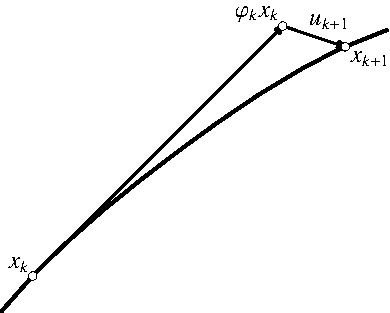
\includegraphics{images/filter-1.pdf}
\caption{Systementwicklung durch die Abbildung $\varphi_k$, der Vektor $u_k$
gibt die Unzulänglichkeiten des durch $\varphi_k$ beschriebenen Modells
wieder.
\label{filter-systementwicklung}}
\end{figure}
In der Realität bewegt sich das System kaum genau nach diesen Gleichungen.
Vielmehr wird es von äusseren Störungen beeinflusst, die sich einer
exakten Vorhersage entziehen, wir tragen dem Rechnung mit Hilfe eines
zusätzlichen Zufallsvektors $u_k$ in den Bewegungsgleichungen
\[
x_{k+1}=\varphi_kx_k+ u_k.
\]
Wir verlangen, dass die Komponenten des Vektors $u_k$ alle unabhängige
Zufallsvariablen sind Erwartungswert 0.
\index{Systemfehler-Kovarianz-Matrix}
\index{Systemfehler!Kovarianz-Matrix}
Die Kovarianz-Matrix $Q_k=E(u_k\cdot u_k^t)$ ist
ein Mass dafür.
$u_k$ heisst auch Prozessrauschen oder Systemfehler.

Die Messfehler modellieren wir durch einen
Zufallsvektor $w_k$, der bei jeder Messung dazukommt, also
\[
z_k=H_kx_k+w_k.
\]
Die Komponenten von $w_k$ sollen unabhängige Zufallsvariablen mit
Erwartungswert $0$ sein, d.~h.~es liegen keine systematischen Messfehler
vor.
Dies bedeutet, dass die Matrix
\index{Messfehler-Kovarianz-Matrix}
\index{Messfehler!Kovarianz-Matrix}
\[
R_k=E(w_kw_k^t)
\]
Diagonalform hat.
Ausserdem sollen die Messfehler unabhängig vom aktuellen Zustand
sein, in Matrix-Form können wir dies durch $E(x_kw_k^t)=0$ ausdrücken.
Man nennt $w_k$ oft auch das Messrauschen.

Die Messfehler $w_k$ und das Prozessrauschen $u_k$ sollen ebenfalls unabhängig
sein, also $E(w_ku_k^t)=0$.

Das Filterproblem besteht darin, aus den bekannten Messwerten von $z_0,\dots,z_k$
die bestmögliche Schätzung $\hat x_k$ zu ermitteln.
Dabei sollen
natürlich die Bewegungsgleichungen berücksichtigt werden.
Da aber
mit der Matrix $R_k$ auch die Grössenordnung der Messfehler bekannt ist,
sollen ``schlechte'' Messwerte geringeres Gewicht erhalten also gute
Messwerte.
Je mehr Werte $z_k$ bekannt werden, desto besser sollte die
Schätzung werden.

In einer praktischen Realisierung muss aber auch die Berechnung der Schätzung
einfach und mit wenig Speicherplatz möglich sein.
Insbesondere sollte zur
Berechnung der neuen Schätzung $\hat x_{k+1}$ nur der letzte bekannte Schätzwert
$\hat x_k$ und die Messung $z_{k+1}$ notwendig sein.
Ausserdem soll der Schätzer
$\hat x_k$ möglichst gut sein, d.~h.~erwartungstreu, linear, iterativ und
mit minimaler Varianz.

\begin{definition}Gegeben ist ein lineares System mit der Zeitentwicklung
\[
x_{k+1}=\varphi_kx_k+u_k,
\]
wobei $x_k$ und $u_k$ unabhängigen Zufallsvariablen sind,
$u_k$ mit Erwartungswert $0$ und bekannter Kovarianzmatrix $Q_k$, d.~h.
\[
E(u_kx_k^t)=0,\qquad E(u_k)=0,\qquad E(u_ku_k^t)=Q_k.
\]
An diesem System werden Beobachtungen
\[
z_k=H_kx_k+w_k
\]
vorgenommen, $w_k$ sind mit $x_k$ und $u_k$ unabhängige Zufallsvariablen
$w_k$ mit Erwartungswert $0$ und bekannter Kovarianzmatrix $R_k$, also
\[
E(w_kx^t)=0,\qquad E(w_k)=0,\qquad E(w_kw_k^t)=R_k.
\]
Das Filterproblem besteht darin, einen Schätzer $\hat x_k$ zu
finden, welcher sich linear aus $\hat x_{k-1}$ und $z_k$ berechnen lässt.
Die Fehler $\tilde x_k=\hat x_k-x_k$ können mit der Fehlerkovarianzmatrix
\[
P_k=E(\tilde x_k\tilde x_k^t)
\]
gemessen werden.
Der Schätzer soll so gewählt werden, dass die Spur
$\operatorname{tr}P_k$ minimal wird.
\end{definition}

